\documentclass[aspectratio=169,xcolor=dvipsnames]{beamer}
\usetheme{Pittsburgh}
\usepackage{xcolor}
\usepackage[utf8]{inputenc}
\usepackage[german]{babel}
\usepackage{amsmath}
\usepackage{amsfonts}
\usepackage{amssymb}
\usepackage{graphicx}
\usepackage{multicol}
\usepackage{wrapfig}
\usepackage{hyperref}
\usepackage{tikz}
\usepackage{enumitem}
\usepackage{xcolor}
\usepackage{scalerel,xparse}

\usetikzlibrary{shapes,arrows,chains}

\author{Jonas Betzendahl}
\title{Meine Kollegin -- Ein Roboter?}

\beamertemplatenavigationsymbolsempty 
\setbeamercolor{frametitle}{fg=Red}

%src: https://tex.stackexchange.com/questions/34921/how-to-overlap-images-in-a-beamer-slide
\def\Put(#1,#2)#3{\leavevmode\makebox(0,0){\put(#1,#2){#3}}}

\begin{document}

\NewDocumentCommand\emojieu{}{
    \scalerel*{
        
\includegraphics{images/flag-european-union.png}
    }{X}
}

%------------------------------------------------------------------------------------
\section{Einführung}
\usebackgroundtemplate{
\includegraphics[height=\paperheight,width=\paperwidth]{images/background_title}}

\begin{frame}
\begin{center}
\vfill
\huge Meine Kollegin -- Ein Roboter?
\normalsize 
\smallskip
\smallskip

Künstliche Intelligenz in Theorie und Praxis
\bigskip\bigskip

\large Jonas Betzendahl, M.Sc.\\\normalsize FAU Erlangen-Nürnberg
\bigskip\bigskip\large

\href{https://twitter.com/lambdatotoro}{
\includegraphics[scale=0.125]{images/twitter_logo.png}}
\href{https://chaos.social/@lambdatotoro}{\includegraphics[scale=0.125]{images/mastodon_logo.png}}
\href{https://github.com/lambdaTotoro}{
\includegraphics[scale=0.125]{images/github_logo.png}}

\texttt{@lambdaTotoro (@chaos.social)}
\end{center}
\end{frame}

%------------------------------------------------------------------------------------
\usebackgroundtemplate{
\includegraphics[height=\paperheight,width=\paperwidth]{images/background_blank}}

\begin{frame}
\frametitle{Wer bin ich?}
\begin{minipage}{0.6\paperwidth}
\begin{center}
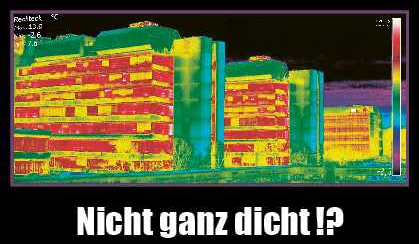
\includegraphics[width=0.8\textwidth,keepaspectratio]{images/thermopostkarte}
\end{center}
\end{minipage}\begin{minipage}{0.25\paperwidth}
\Large
\emph{Jonas Betzendahl}
\normalsize
\bigskip

Kognitive Informatik

Intelligente Systeme
\medskip

WRV @ FAU 
\end{minipage}
\end{frame}

\begin{frame}[fragile]
\frametitle{Wer sind Sie?}
\scriptsize
\begin{minipage}{\textwidth}
\begin{verbatim}
Q: Wie vertraut sind Sie mit dem Thema Künstliche Intelligenz /
   Maschinelles lernen?

A1: Ich bin neu hier / kenne KI nur aus dem TV
A2: Ein paar Grundlagen kenne ich
A3: Ich weiß Bescheid, arbeite aktiv mit KI
A4: Koryphäe auf dem Feld, nur hier um anzugeben
\end{verbatim}
\end{minipage}
\pause \bigskip\bigskip

\begin{minipage}{\textwidth}
\begin{verbatim}
Q: Setzen Sie bereits KI am Arbeitsplatz ein?

A1: Keine KI notwendig, nur aus Interesse hier
A2: Wüsste gerne ob das für uns Sinn ergibt
A3: Wir planen das in Zukunft einzuführen
A4: KI ist bei uns schon längst im Einsatz
\end{verbatim}
\end{minipage}
\end{frame}

\begin{frame}
\frametitle{Motivation}
\begin{center}
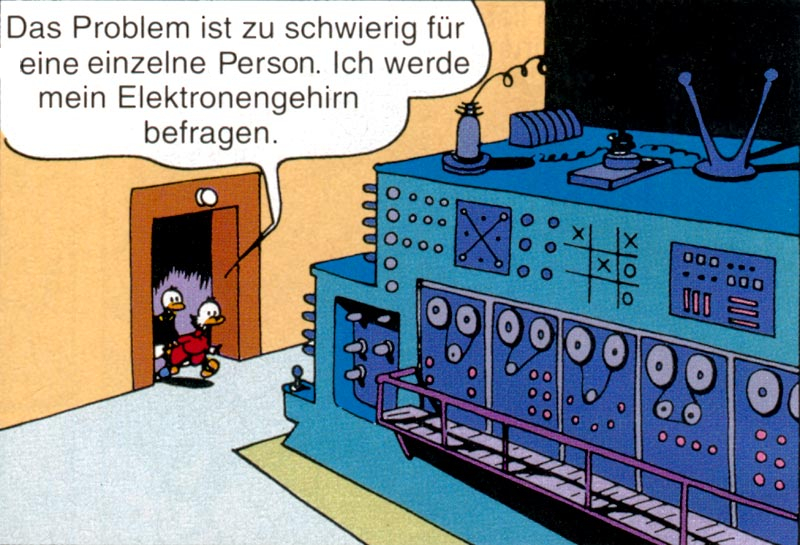
\includegraphics[height=0.75\paperheight,keepaspectratio]{images/elektronengehirn} 
\end{center}
\end{frame}

\section{Grundlagen}

\begin{frame}
\frametitle{\glqq Algorithmen\grqq}
\begin{center}

\includegraphics[height=0.75\paperheight,keepaspectratio]{images/man-cooking-clipart} 
\end{center}
\end{frame}

\begin{frame}
\frametitle{\glqq Maschinelles Lernen\grqq}
\begin{center}

\includegraphics[height=0.7\paperheight,keepaspectratio]{images/funnel} 
\end{center}
\end{frame}

\begin{frame}
\frametitle{\glqq Künstliche Intelligenz\grqq}
\begin{minipage}{0.5\paperwidth}
\begin{center}

\includegraphics[height=0.6\paperheight,keepaspectratio]{images/man-shrug} 
\end{center}
\end{minipage}\begin{minipage}{0.3\paperwidth}
\Large
\begin{itemize}
\item Inferenz?
\item Objekterkennung?
\item Schach? Go?
\item Auto fahren?
\item Emotionen?
\item \dots
\end{itemize}
\end{minipage}
\end{frame}

\begin{frame}
\frametitle{Wo anfangen?}
\begin{center}
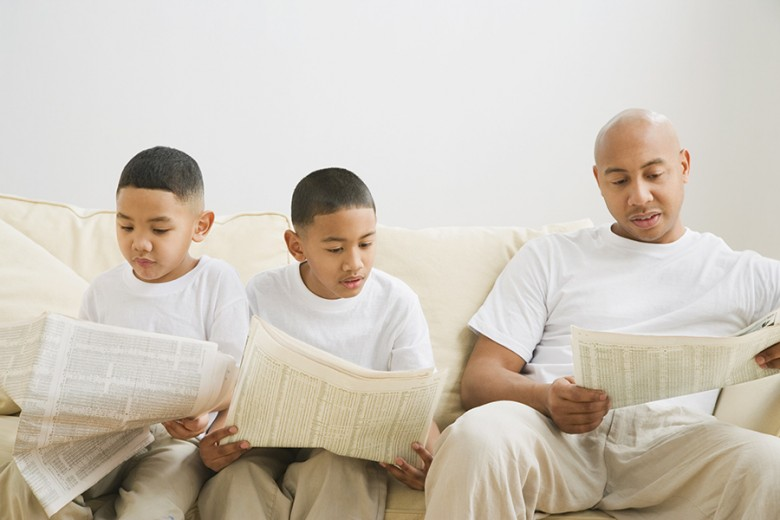
\includegraphics[height=0.7\paperheight,keepaspectratio]{images/imitation} 
\end{center}
\end{frame}

\begin{frame}
\frametitle{Neuron}
\begin{center}

\includegraphics[height=0.82\paperheight,keepaspectratio]{images/neuron} 
\end{center}
\end{frame}

\begin{frame}
\frametitle{Perzeptron}
\begin{center}
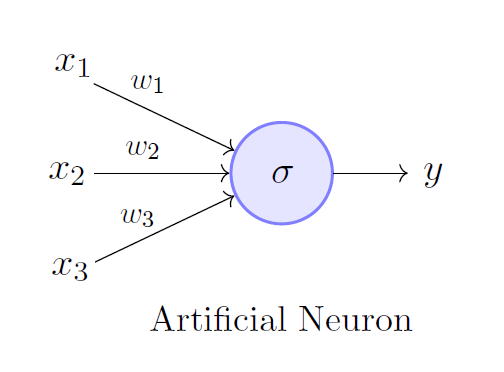
\includegraphics[height=0.82\paperheight,keepaspectratio]{images/perceptron} 
\end{center}
\end{frame}

\begin{frame}
\begin{center}
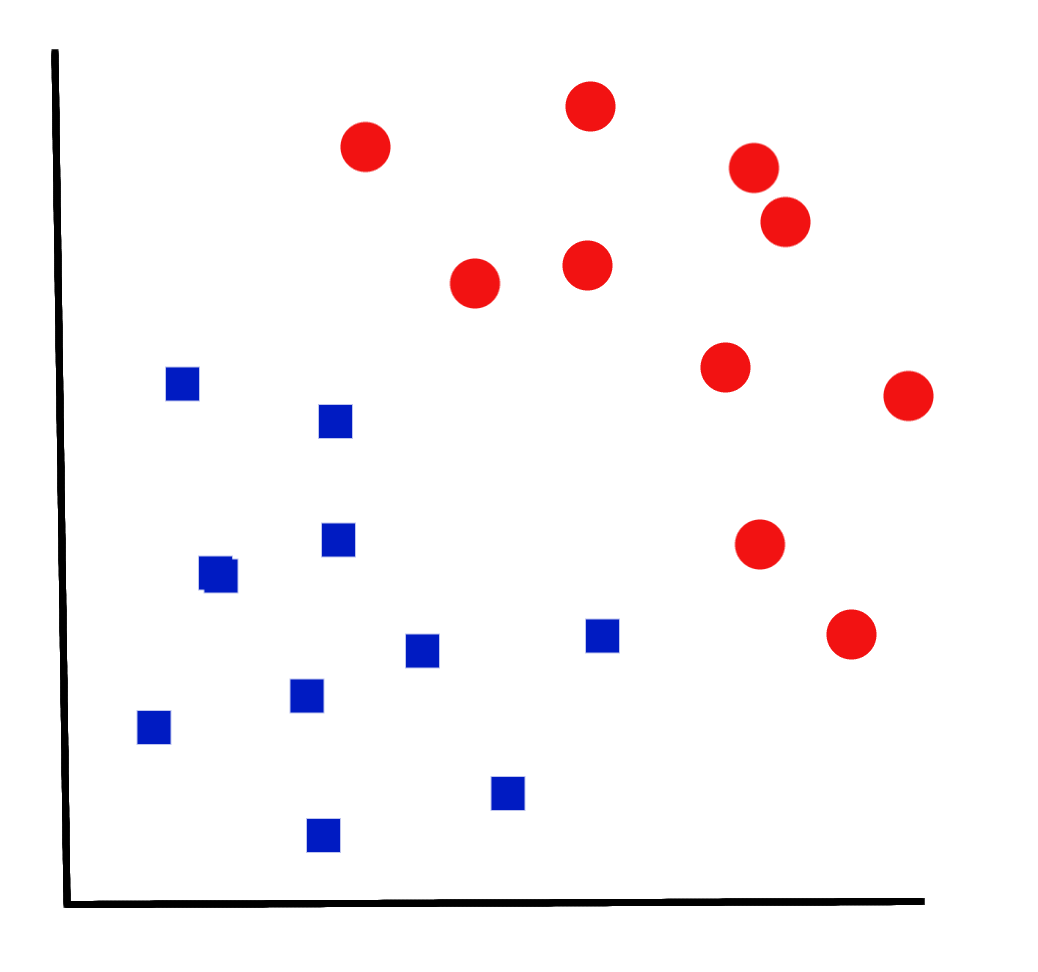
\includegraphics[height=0.8\paperheight,keepaspectratio]{images/coordinates_points_empty} 
\end{center}
\end{frame}

\begin{frame}
\begin{center}
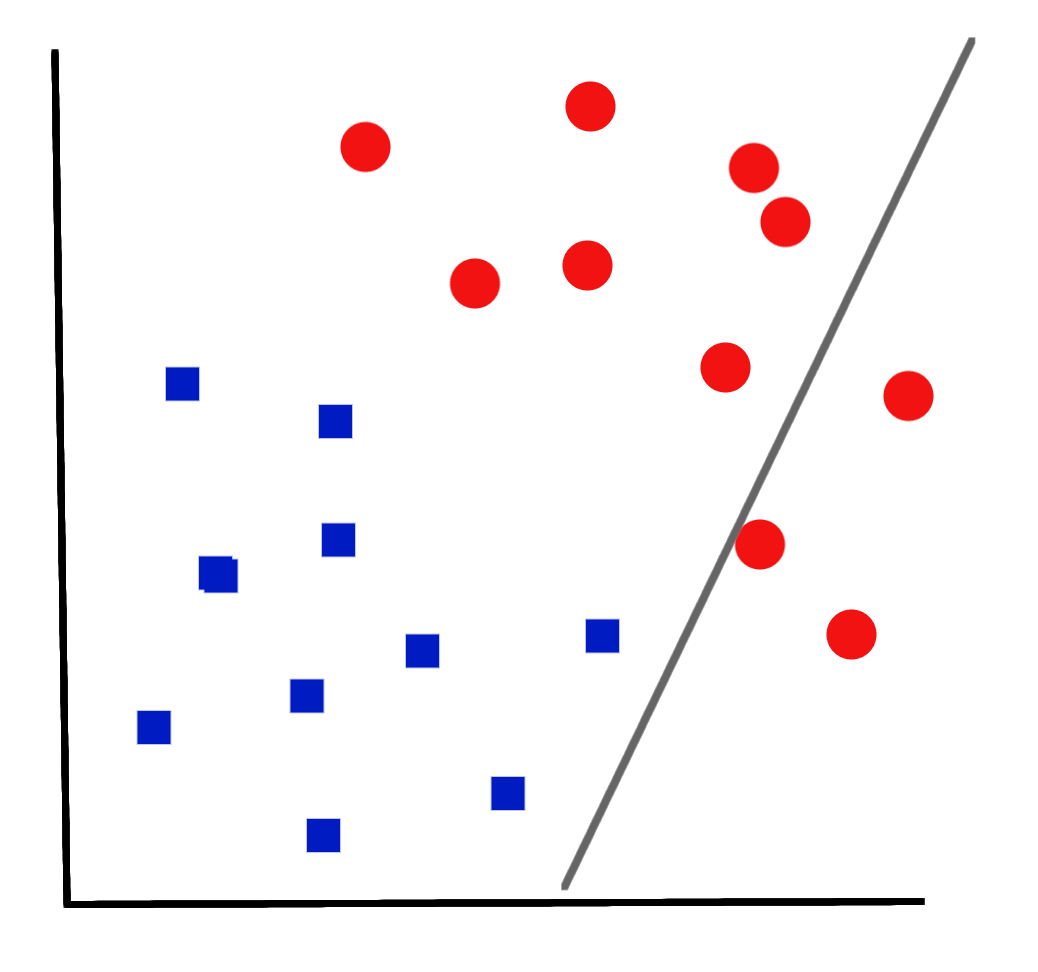
\includegraphics[height=0.8\paperheight,keepaspectratio]{images/coordinates_points_1} 
\end{center}
\end{frame}

\begin{frame}
\begin{center}
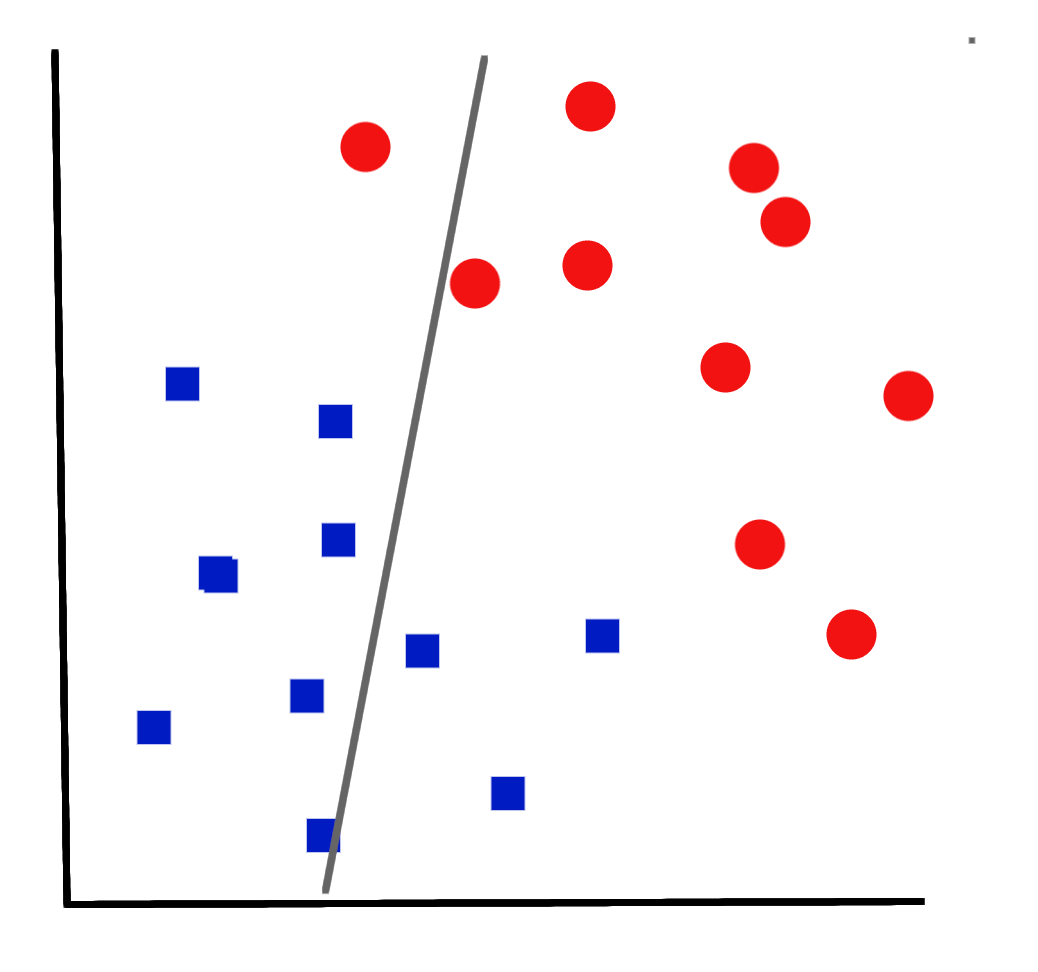
\includegraphics[height=0.8\paperheight,keepaspectratio]{images/coordinates_points_2} 
\end{center}
\end{frame}

\begin{frame}
\begin{center}
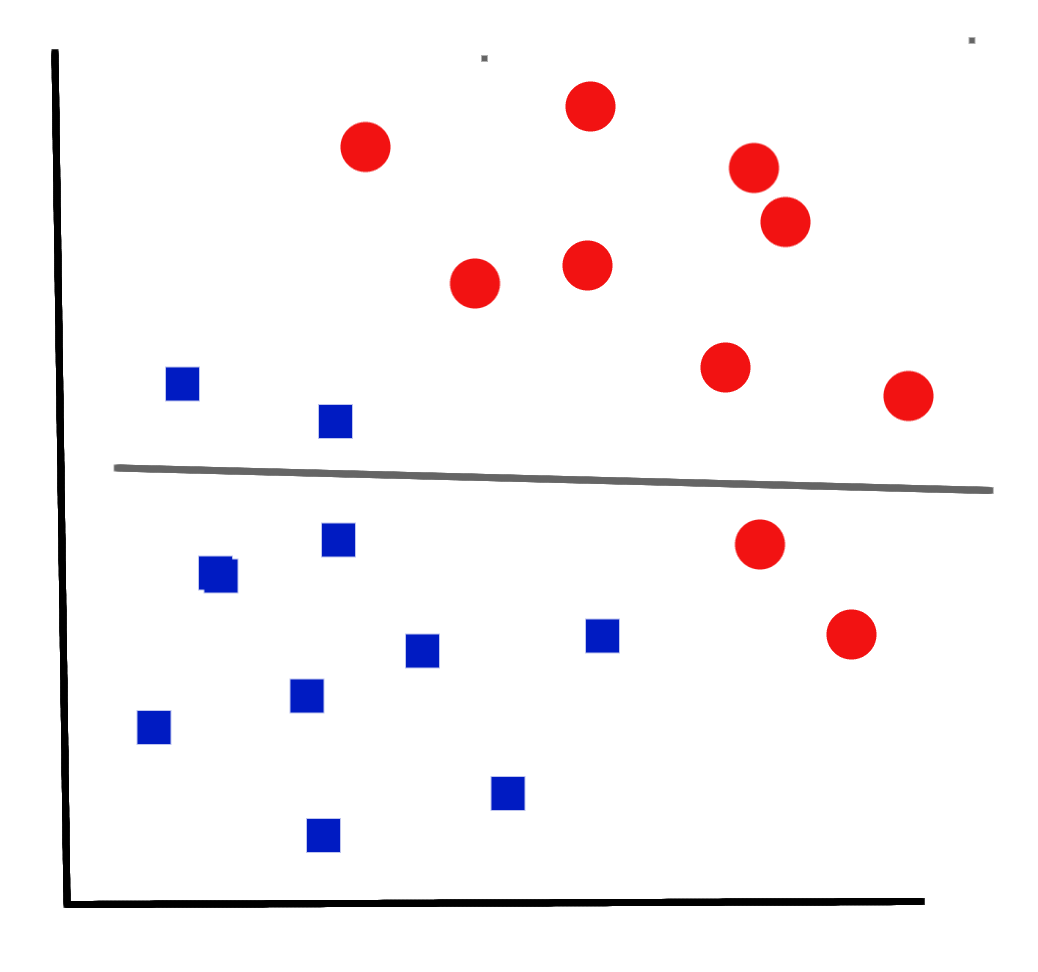
\includegraphics[height=0.8\paperheight,keepaspectratio]{images/coordinates_points_3} 
\end{center}
\end{frame}

\begin{frame}
\begin{center}
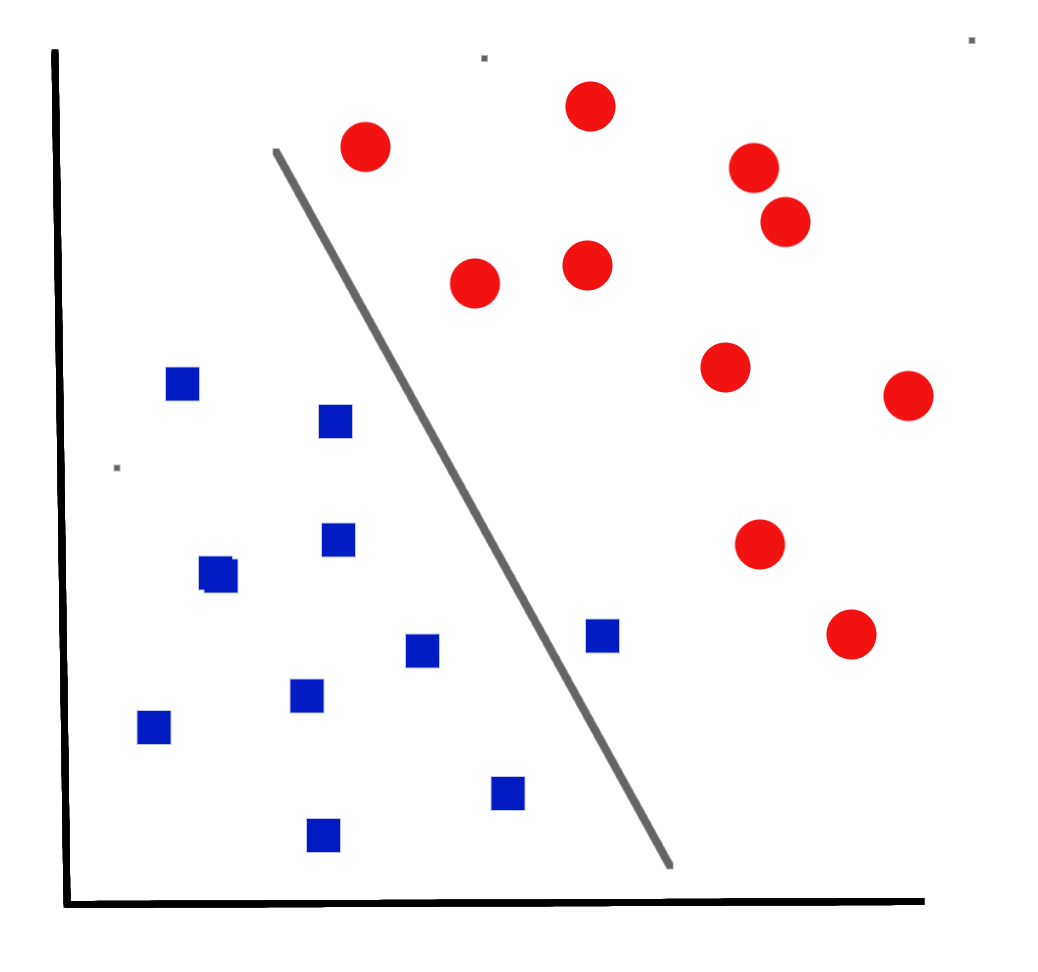
\includegraphics[height=0.8\paperheight,keepaspectratio]{images/coordinates_points_4} 
\end{center}
\end{frame}

\begin{frame}
\begin{center}
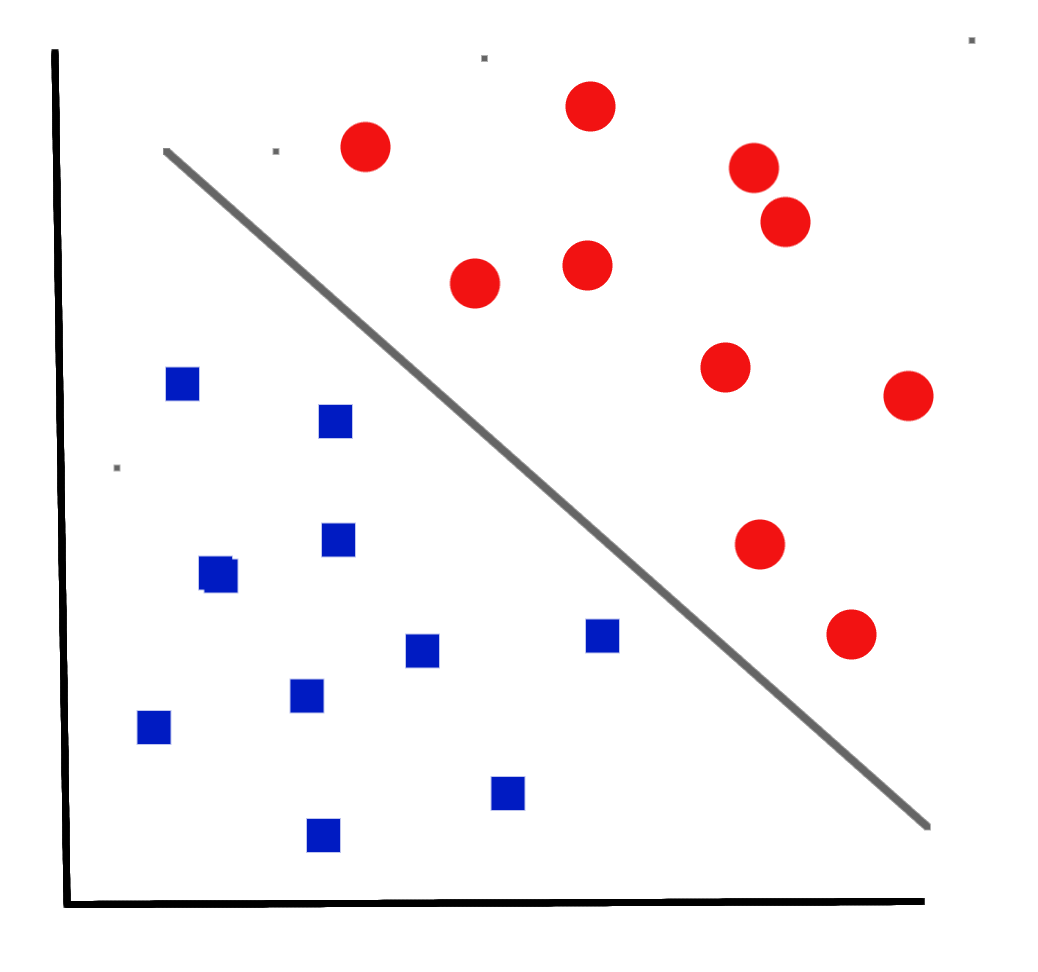
\includegraphics[height=0.8\paperheight,keepaspectratio]{images/coordinates_points_5} 
\end{center}
\end{frame}

\begin{frame}
\begin{center}
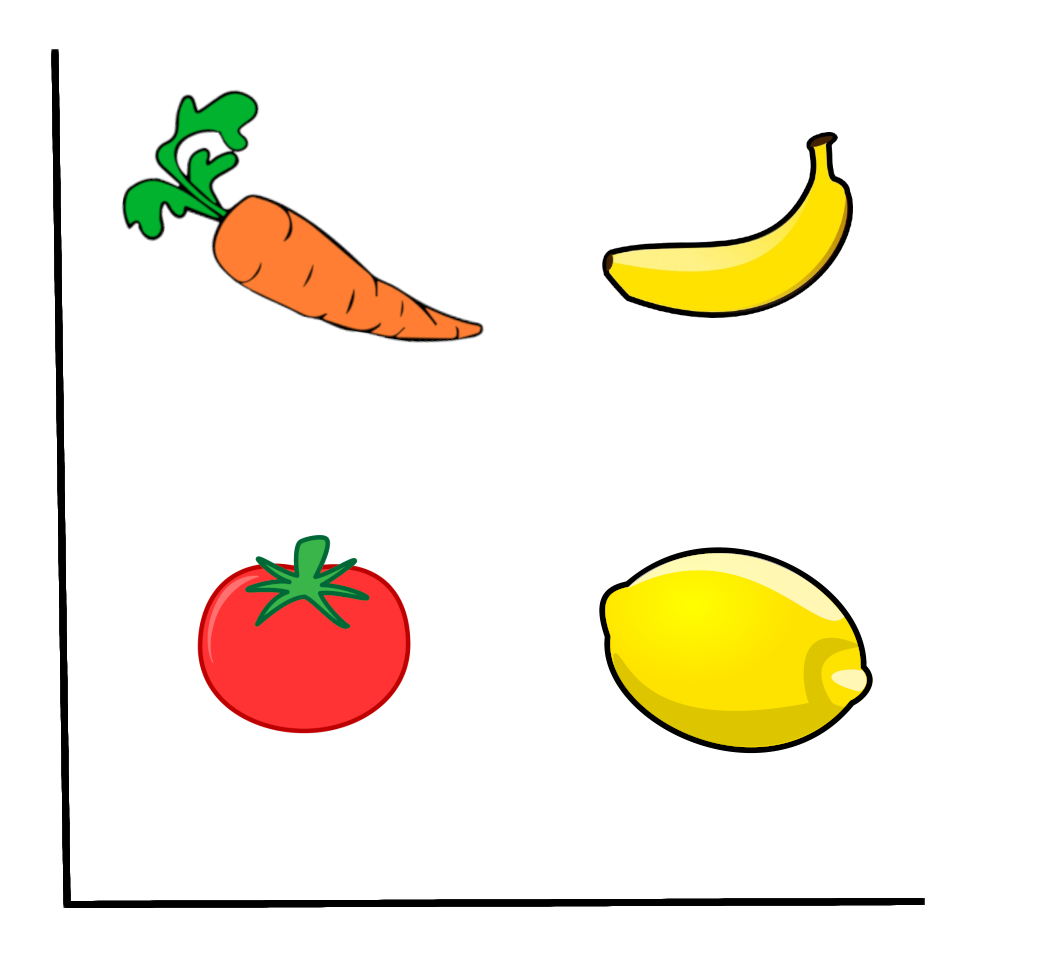
\includegraphics[height=0.8\paperheight,keepaspectratio]{images/coordinates_veggi_empty} 
\end{center}
\end{frame}

\begin{frame}
\begin{center}
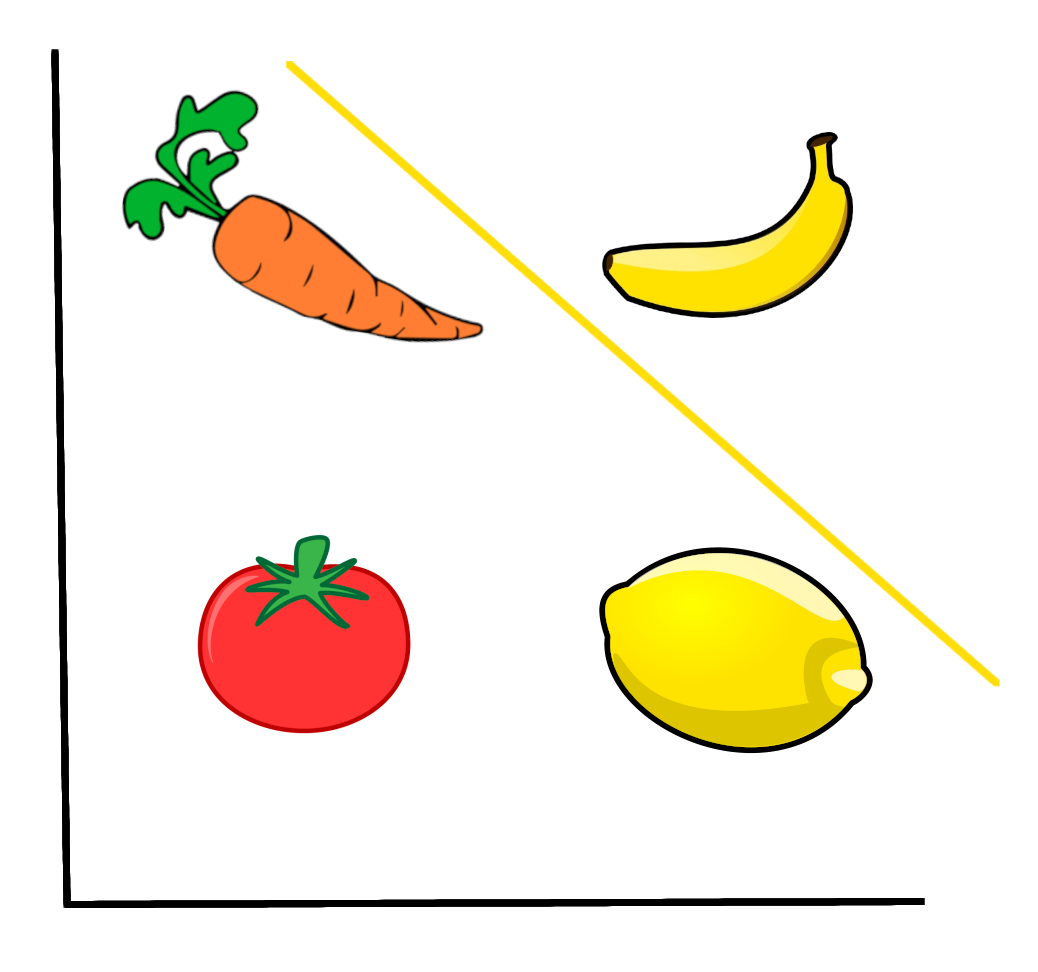
\includegraphics[height=0.8\paperheight,keepaspectratio]{images/coordinates_veggi_line} 
\end{center}
\end{frame}

\usebackgroundtemplate{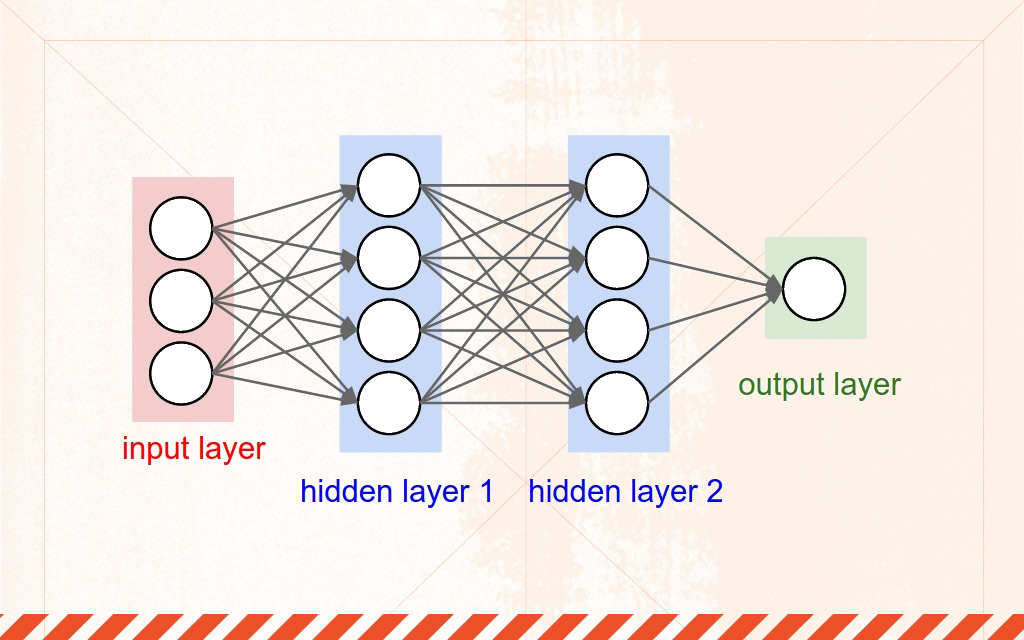
\includegraphics[height=\paperheight,width=\paperwidth]{images/background_nn}}

\begin{frame}
\end{frame}

\usebackgroundtemplate{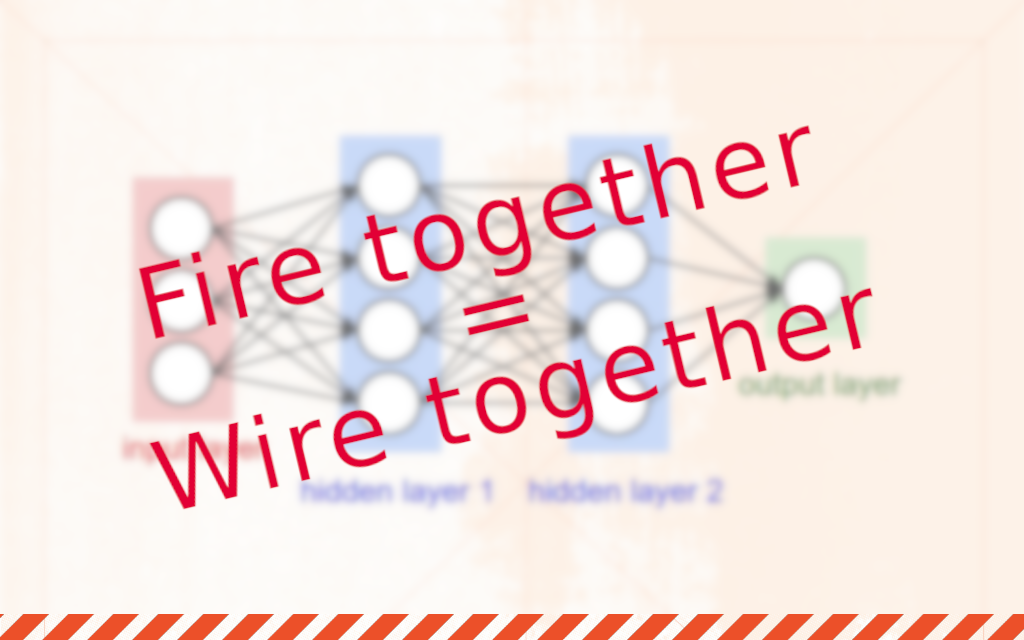
\includegraphics[height=\paperheight,width=\paperwidth]{images/background_nn_fw}}

\begin{frame}
\end{frame}

\usebackgroundtemplate{
\includegraphics[height=\paperheight,width=\paperwidth]{images/background_blank}}

%----------------------------------------------

\section{Fallstudien}

\begin{frame}
\begin{center}

\includegraphics[height=0.65\paperheight,keepaspectratio]{images/no_bias} 
\end{center}
\end{frame}

\begin{frame}[fragile]
\begin{verbatim}
     "Human beings, who are almost unique in having the
     ability to learn from the experience of others, are also
     remarkable for their apparent disinclination to do so."
     
                                            (Douglas Adams)
\end{verbatim}
\end{frame}

\begin{frame}
\frametitle{Adversarial Objects (1)}
\begin{center}
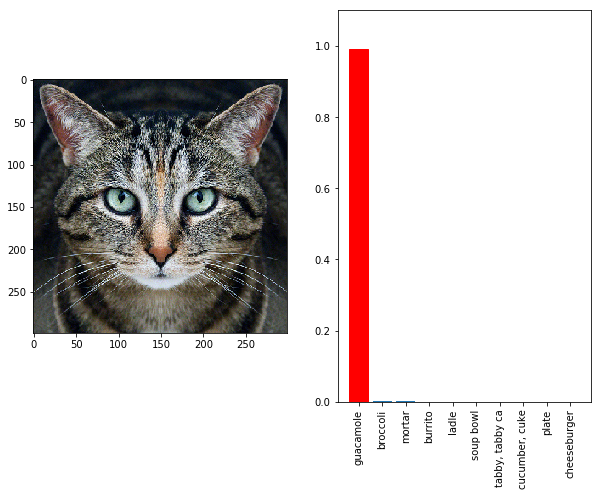
\includegraphics[height=0.7\paperheight,keepaspectratio]{images/cat_adversarial} 
\end{center}
\end{frame}

\begin{frame}
\frametitle{Adversarial Objects (2)}
\begin{center}
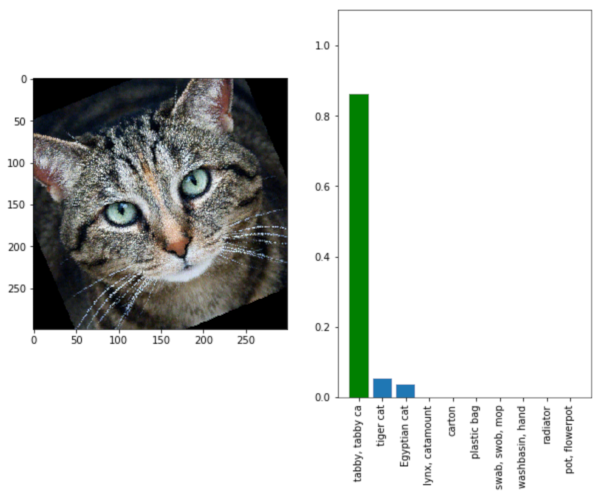
\includegraphics[height=0.7\paperheight,keepaspectratio]{images/cat_rotated} 
\end{center}
\end{frame}

\begin{frame}
\frametitle{Adversarial Objects (3)}
\begin{center}
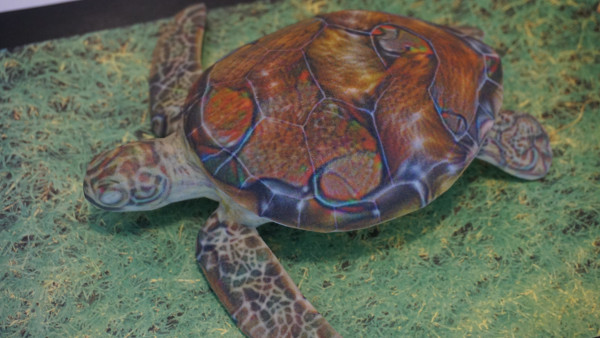
\includegraphics[height=0.7\paperheight,keepaspectratio]{images/rifle_turtle} 
\end{center}
\end{frame}

\begin{frame}
\frametitle{Adversarial Objects (4)}
\begin{center}
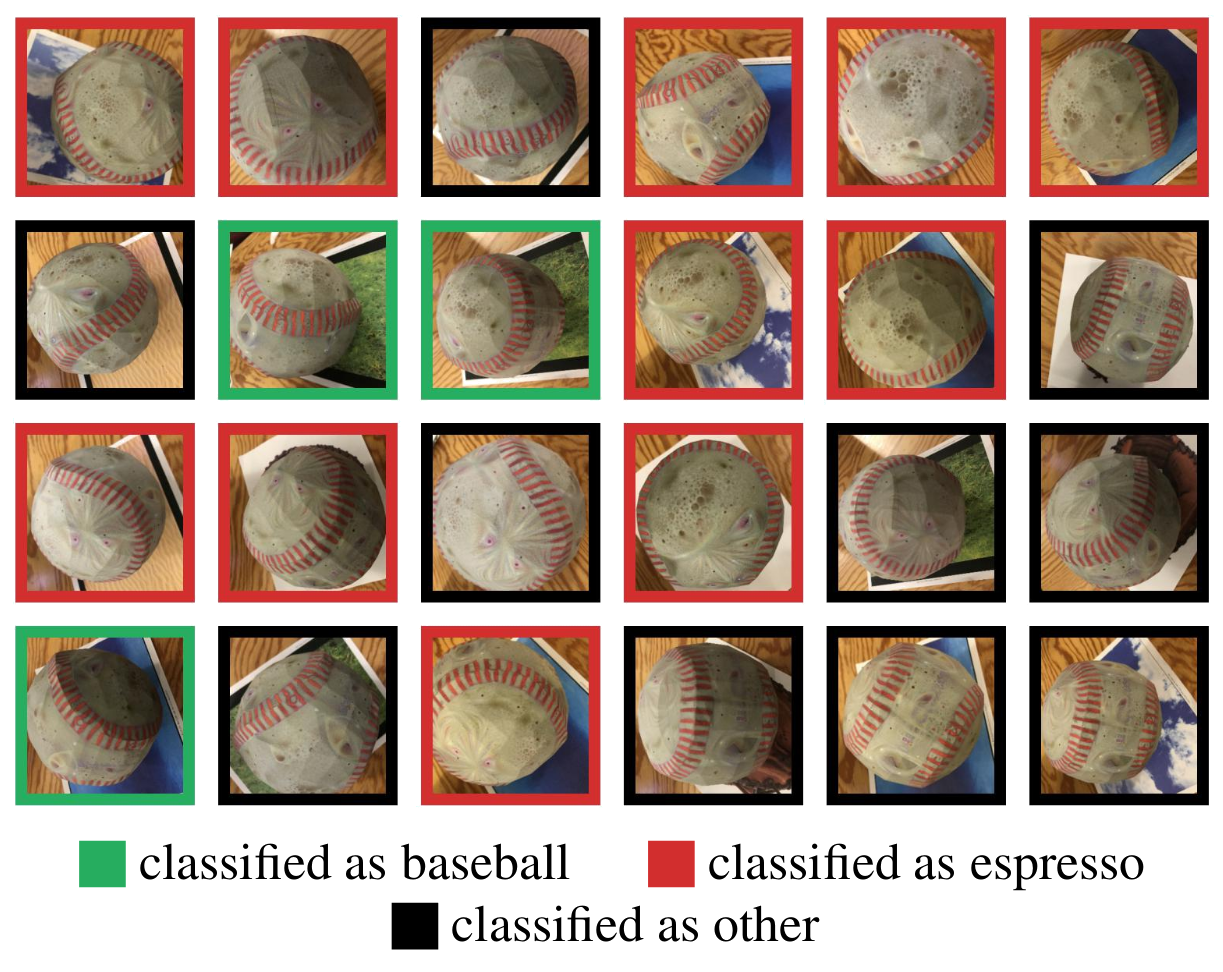
\includegraphics[height=0.7\paperheight,keepaspectratio]{images/baseball_class} 
\end{center}
\end{frame}

\begin{frame}
\frametitle{Entpixelisierung (1)}
\begin{center}
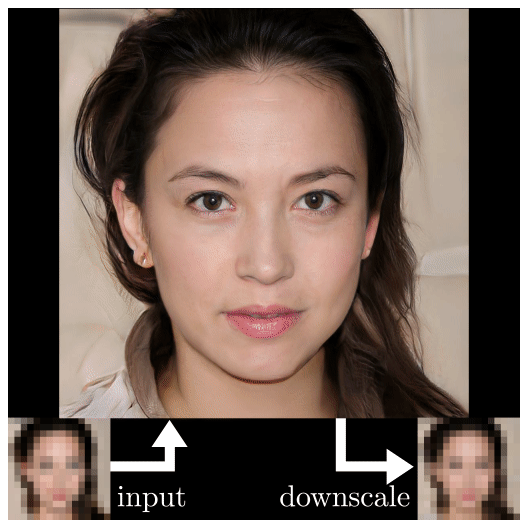
\includegraphics[height=0.7\paperheight,keepaspectratio]{images/example_depixelise} 
\end{center}
\end{frame}

\begin{frame}
\frametitle{Entpixelisierung (2)}
\begin{minipage}{0.45\textwidth}
\begin{center}
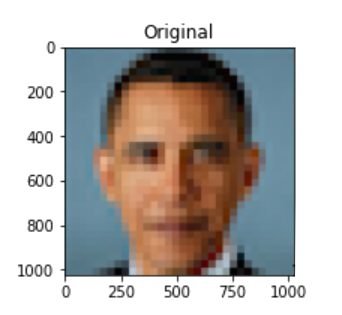
\includegraphics[height=0.7\paperheight,keepaspectratio]{images/obama_depixelise1} 
\end{center}
\end{minipage}\pause \begin{minipage}{0.45\textwidth}
\begin{center}
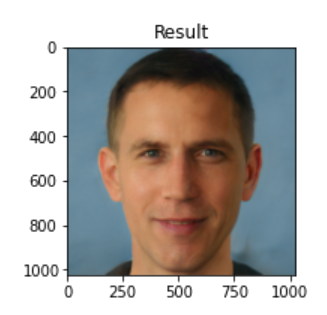
\includegraphics[height=0.7\paperheight,keepaspectratio]{images/obama_depixelise2} 
\end{center}
\end{minipage}
\end{frame}

\begin{frame}
\frametitle{Phrenologie, aber vom Computer}
\begin{minipage}{.455\textwidth}
\begin{center}
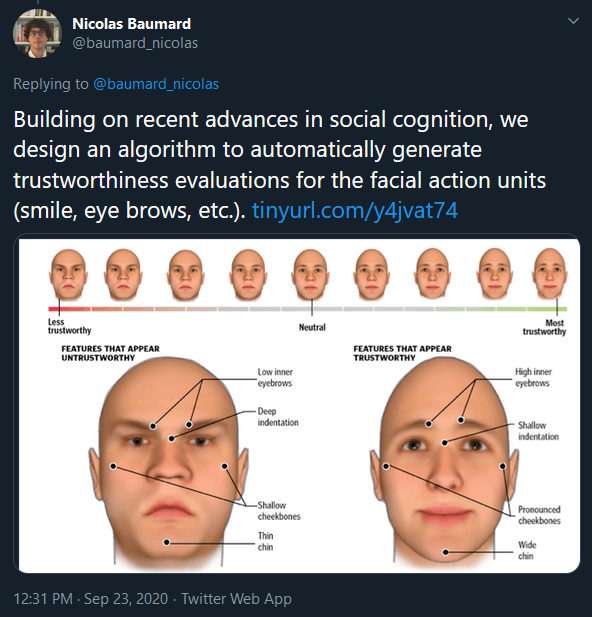
\includegraphics[width=0.9\textwidth, keepaspectratio]{images/phrenology.png}
\end{center}
\end{minipage}\begin{minipage}{.545\textwidth}
\begin{center}
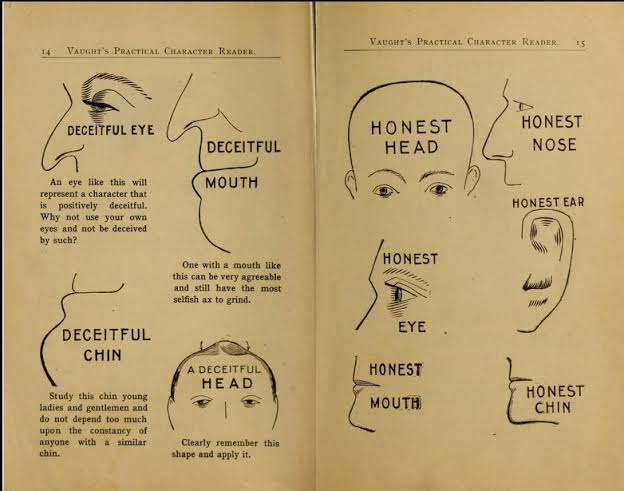
\includegraphics[width=0.99\textwidth, keepaspectratio]{images/phrenology.jpg}
\end{center}
\end{minipage}
\end{frame}

\begin{frame}
\frametitle{Genderify}
\begin{center}
Please don't try to guess things that can't be guessed.
\end{center}
\end{frame}

\begin{frame}
\frametitle{Amazon / Arbeitsmarkt in Österreich}
\begin{center}
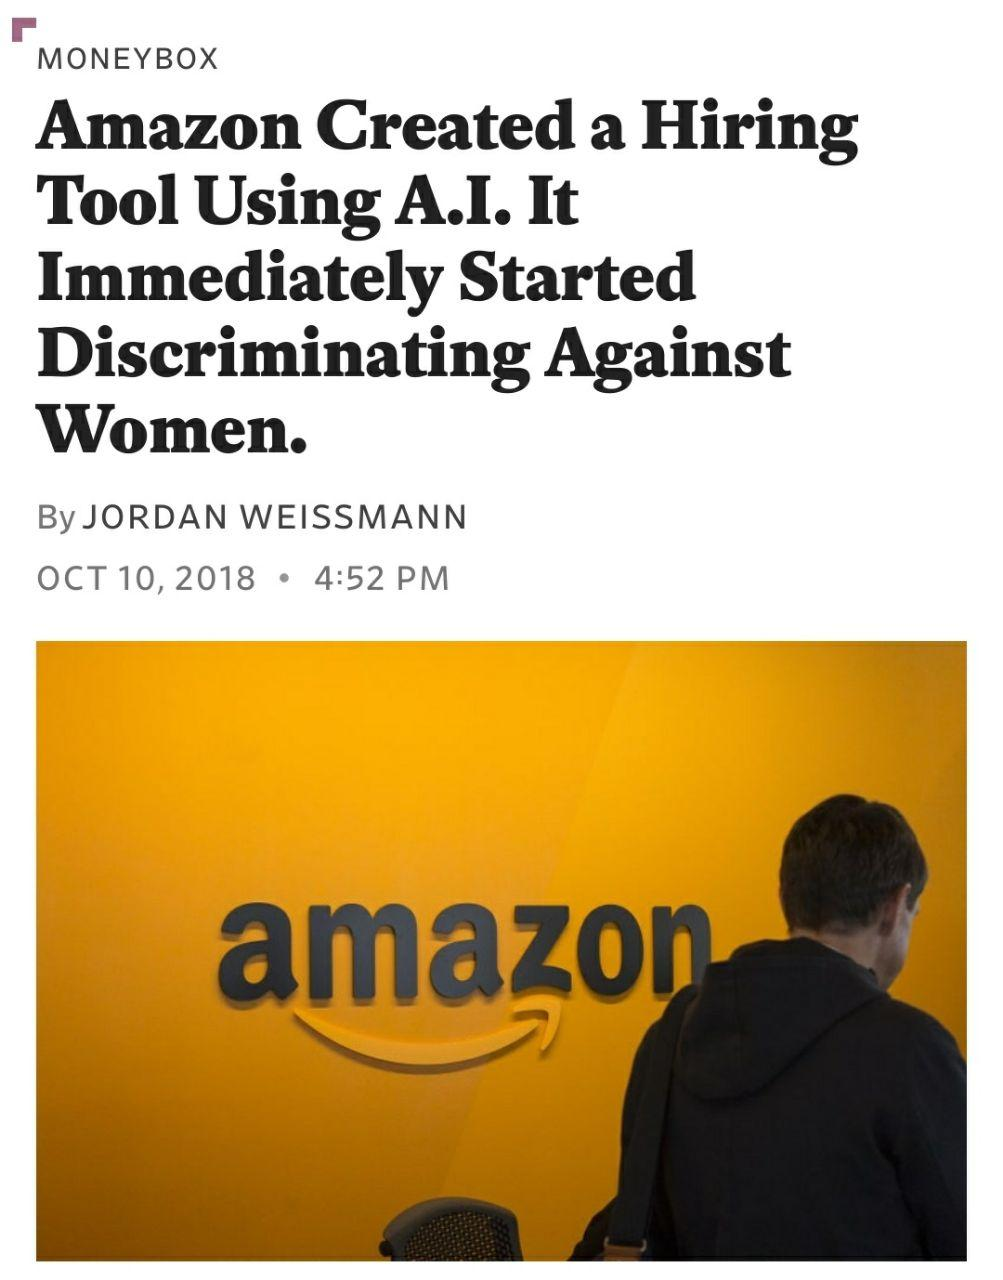
\includegraphics[height=0.7\paperheight,keepaspectratio]{images/amazon_hiring} 
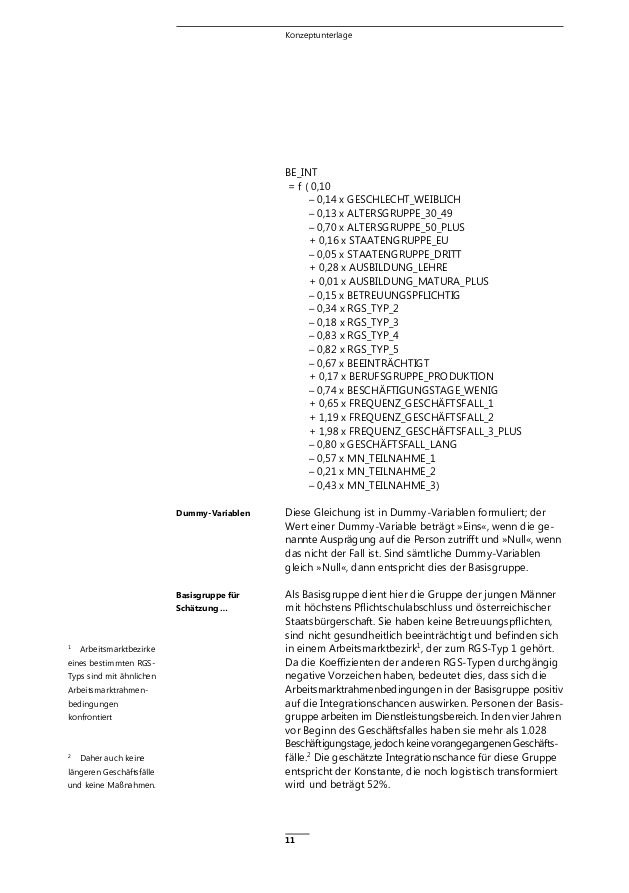
\includegraphics[height=0.7\paperheight,keepaspectratio]{images/negativfaktor} 
\end{center}
\end{frame}

\begin{frame}
\frametitle{Unintended Consequences}
\begin{center}

\includegraphics[height=0.7\paperheight,keepaspectratio]{images/youtube} 
\end{center}
\end{frame}

\begin{frame}
\frametitle{Selbsterfüllende Prophezeihungen}
\begin{center}
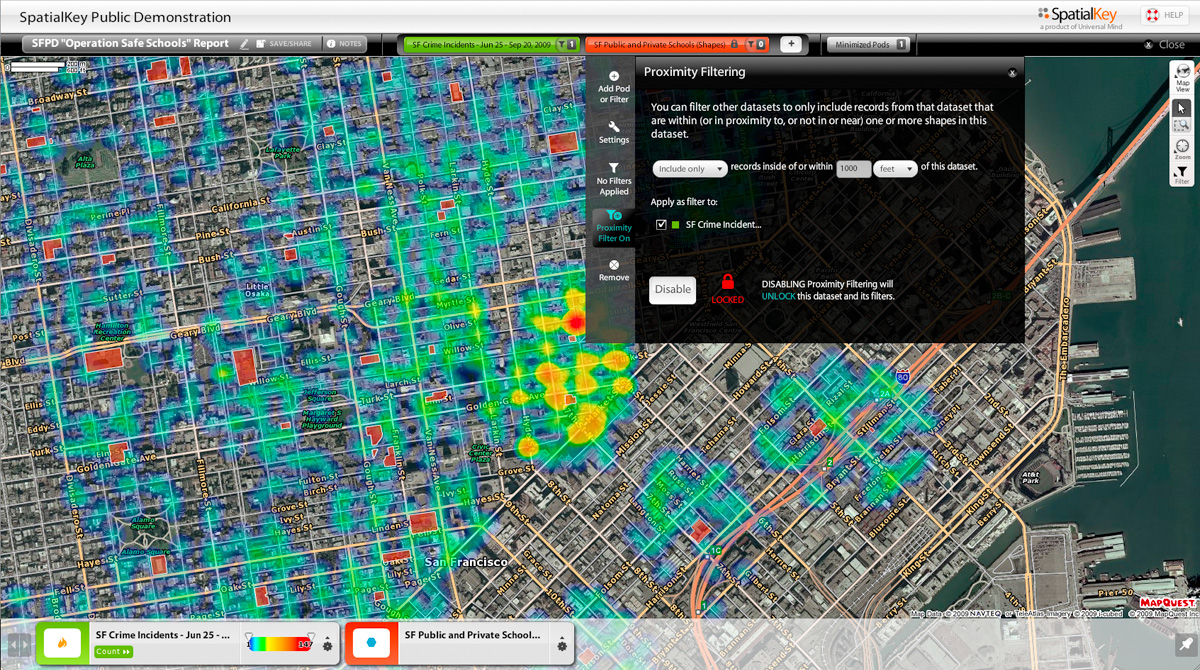
\includegraphics[height=0.7\paperheight,keepaspectratio]{images/predictive_policing} 
\end{center}
\end{frame}

\begin{frame}
\frametitle{Predictive Maintenance}
\begin{center}
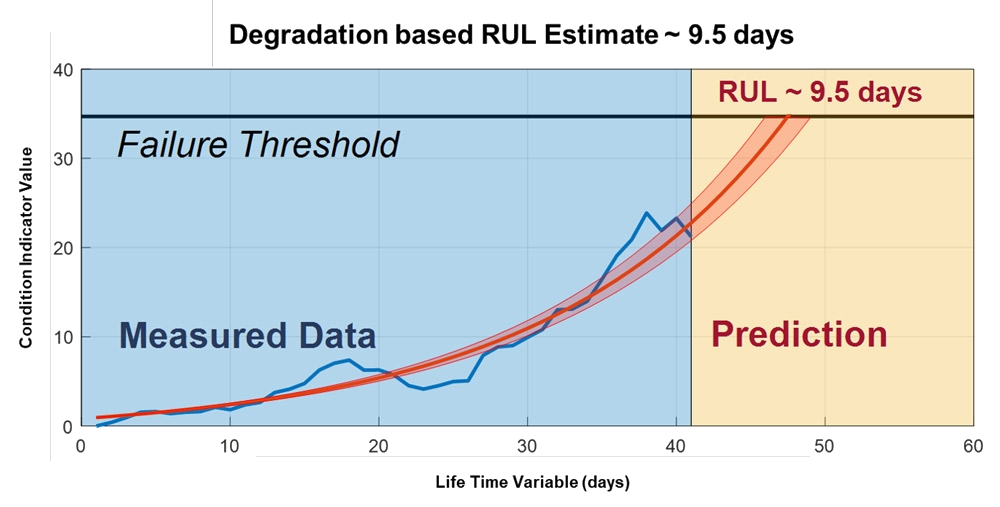
\includegraphics[height=0.7\paperheight,keepaspectratio]{images/rul_threshold} 
\end{center}
\end{frame}

\section{Richtlinien}

\begin{frame}
\begin{center}

\includegraphics[height=0.7\paperheight,keepaspectratio]{images/quo-vadis} 
\end{center}
\end{frame}

\begin{frame}
\frametitle{Verschiedenste Ansätze}
\begin{center}
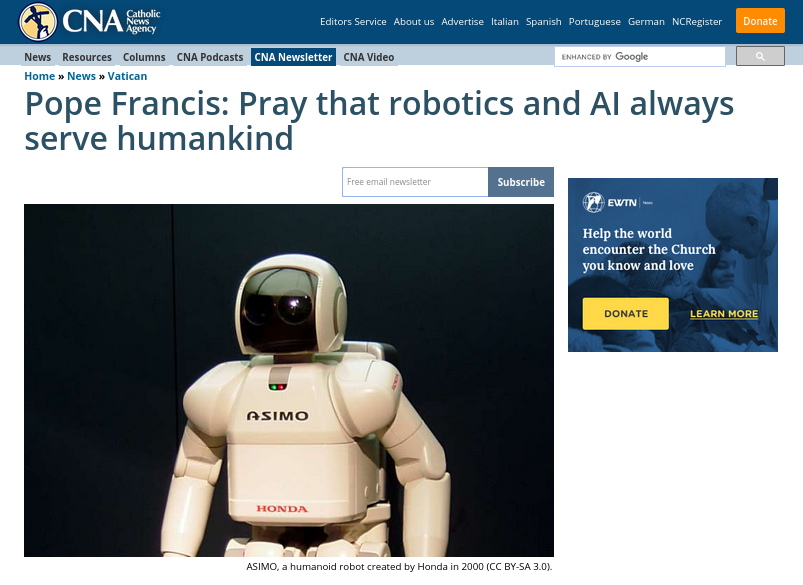
\includegraphics[height=0.7\paperheight,keepaspectratio]{images/pope_pray} 
\end{center}
\end{frame}


\begin{frame}[fragile]
\frametitle{Nicht alles Ethik was glänzt}
\begin{center}
Das Institut für ethisches Maschine Learning schlägt folgende Richtlinien vor:
\end{center}
\medskip

\large
\setlength{\leftmargini}{150pt}
\begin{itemize}[label=\textcolor{RedOrange}{\textbullet}]
\item Human Augmentation
\item Bias Evaluation
\item Explainability by Justification 
\item Reproducible Operations
\item Displacement Strategy
\item Practical Accuracy
\item Trust by Privacy
\item Data Risk Awareness
\end{itemize}
\end{frame}

\usebackgroundtemplate{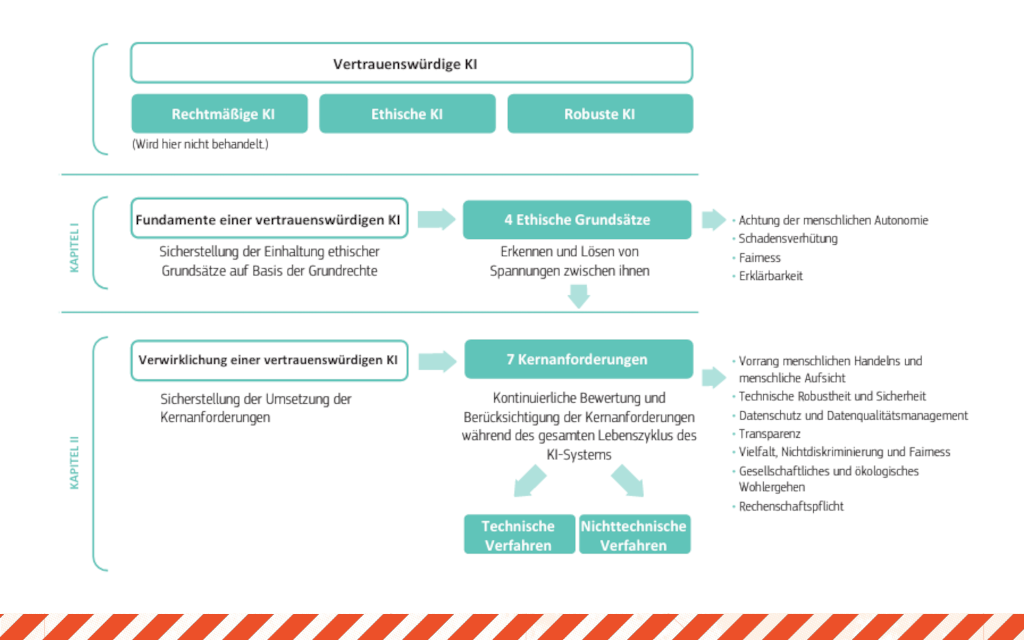
\includegraphics[height=\paperheight,width=\paperwidth]{images/background_eu}}

\begin{frame}
\end{frame}

\usebackgroundtemplate{
\includegraphics[height=\paperheight,width=\paperwidth]{images/background_blank}}

\begin{frame}
\begin{center}
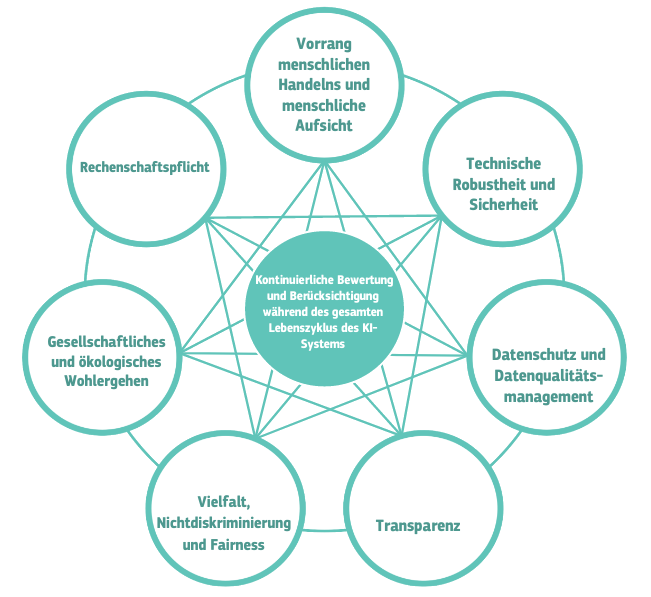
\includegraphics[height=0.75\paperheight,keepaspectratio]{images/eu_prinzipien} 
\end{center}
\end{frame}

\section{Schluss}
\scriptsize
\begin{frame}[fragile]
\frametitle{Ausblick}
\begin{minipage}{\textwidth}
\begin{verbatim}
Q: Falls Sie aktuell (noch) keine KI einsetzen:
   Was denken Sie nach diesem Vortrag über die Möglichkeit?

A1: Macht bei uns nach wie vor keinen Sinn
A2: Geringerer Enthusiasmus als vorher
A3: Gleicher Enthusiasmus als vorher
A4: Größerer Enthusiasmus als vorher
\end{verbatim}
\end{minipage}
\pause\bigskip\bigskip

\begin{minipage}{\textwidth}
\begin{verbatim}
Q: Falls Sie aktuell bereits KI einsetzen:
   Was denken Sie nach diesem Vortrag über Ihre Anwendung?

A1: Wird morgen abgeschafft, wenn's nach mir geht
A2: Ich glaube, wir sollten nochmal ein paar Dinge überdenken
A3: Nobody's perfect, aber ich glaube wir sind auf gutem Wege
A4: Wir machen sowieso schon alles richtig (hoffentlich) 
\end{verbatim}
\end{minipage}
\end{frame}

\begin{frame}
\frametitle{Quellen}
\small
\begin{center}
\textbf{Diese Präsentation:}\\
\url{github.com/lambdaTotoro/Talks/blob/master/2020-11-04-Stuttgart-MissionM/}
\end{center}
\bigskip

\begin{itemize}
\item EU-Richtlinien: \url{https://ec.europa.eu/futurium/en/ai-alliance-consultation}
\item The Institute for Ethical AI \& Machine Learning: \url{https://ethical.institute/}
\item Awful AI: \url{https://github.com/daviddao/awful-ai}
\item 3Blue1Brown Playlist: \url{www.youtube.com/playlist?list=PLZHQObOWTQDNU6R1_67000Dx_ZCJB-3pi}
\end{itemize}
\end{frame}

\end{document}

